% !TEX root = PREN2_Dokumentation.tex

\section{Projektmanagementplan}

\subsection{Projektorganisation}
\subsubsection{Organisationsplan, Rollen, Zuständigkeiten}
\begin{figure}[H]
    \centering
    %\includegraphics[width=1\textwidth]{bilder/Organigramm.png}
    \caption[Organigramm]{Organigramm\\ Quelle: Autoren}
    \label{img: OrganigrammWiPro}
\end{figure}

\paragraph{Rollen}
\subsubsection{Projektstrukturplan}

\begin{figure}[H]
    \centering
   % 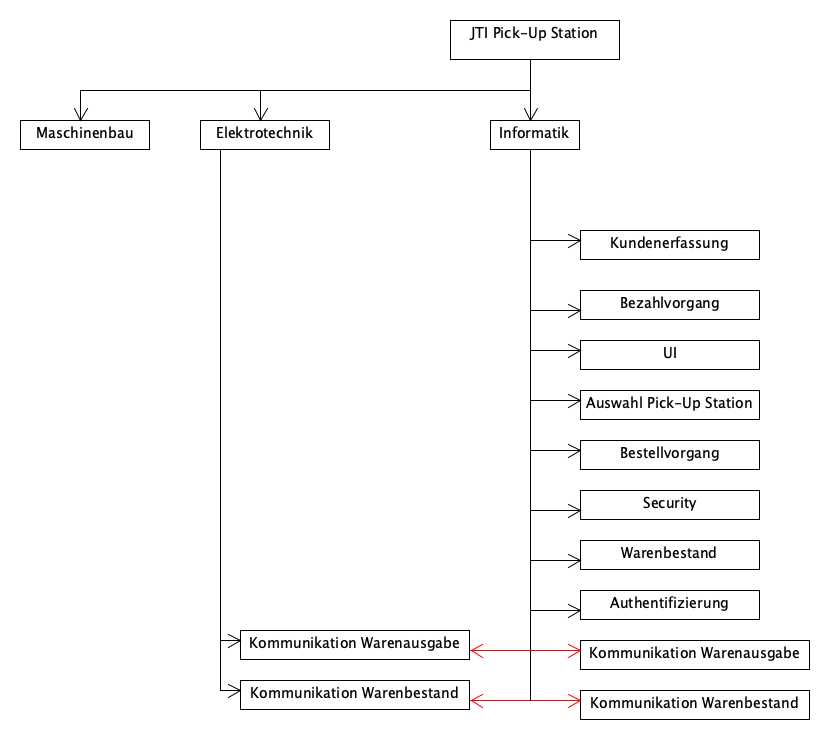
\includegraphics[width=1\textwidth]{bilder/pmp.png}
    \caption[Projektstrukturplan]{Projektstrukturplan,\\ Quelle: Autoren}
    \label{img: Projektstrukturplan}
\end{figure}

\paragraph{Beschreibung}
Im Projektstrukturplan in Abbildung \ref{img: Projektstrukturplan} wird das Projekt in 3 grobe Teile geteilt. Sie sind dabei angepasst an die Grobplanung und decken die Anforderungen ab. 
\newpage
\subsection{Projektführung}
\subsubsection{Rahmenplan}

Im untenstehenden Rahmenplan wird mittels Zeitstrahl eine Grobplanung dargestellt. 

\begin{figure}[H]
    \centering
   % \includegraphics[width=1\textwidth]{bilder/SoDa_Zeitstrahl.png}
    \caption[SoDa Rahmenplan]{Rahmenplan,\\ Quelle: Autoren}
    \label{img: SoDa Rahmenplan}
\end{figure}

Nach 7 absolvierten Sprints wurde der Rahmenplan angepasst. 
\begin{figure}[H]
    \centering
    %\includegraphics[width=1\textwidth]{bilder/Rahmenplan_2.png}
    \caption[SoDa Rahmenplan überarbeitet]{Rahmenplan überarbeitet,\\ Quelle: Autoren}
    \label{img: SoDaRahmenplanUeberarbeitet}
\end{figure}
\newpage
\subsubsection{Meilensteine}\label{Meilensteine}
Wie in Abbildung \ref{img: SoDa Rahmenplan} zu sehen gibt es insgesamt sieben Meilensteine.
Diese werden in folgender Tabelle beschrieben sowie die nötigen Deliverables aufgezeigt.


\begin{table}[H]
\setlength\extrarowheight{2pt} % for a bit of visual "breathing space"
\begin{tabularx}{\textwidth}{|C|C|C|}
\hline
\textbf{Meilenstein} &  \textbf{Beschreibung} & \textbf{Deliverables}  \\

\hline
Projektstart & Bei Meilenstein eins wird das Kickoff-Meeting mit allen Projektteilnehmern durchgeführt. & finale Aufgabenstellung\\

\hline
Start Umsetzung & Bei Meilenstein zwei wird vom klassischen Projektmanagement zum agilen Projektmanagement übergegangen. Dazu muss die Initialisierungsphase abgeschlossen sein& Projektmanagementplan, Systemspezifikation, Anforderungsliste\\

\hline
Abschluss Systemkontext & Zu diesem Zeitpunkt ist alles bereit, um mit der Entwicklung zu beginnen. Es wurden bereits erste GUI Entwürfe erarbeitet sowie die Systemarchitektur definiert.  & CI/CD Umgebung eingerichtet, GUI-Prototyp, UML-Diagramme  
\newline \textbf{Release 1}
\\

\hline
Abschluss Schülermodus & Der Entwicklung des Schülermodus ist abgeschlossen. Es können vorgegebene Fragen beantwortet werden sowie eine Statistik zu bisher Gelerntem eingesehen werden.  & Testprotokolle zu Schülermodus, Demo Schülermodus, Release Schülermodus 
\newline
\textbf{Release 2}
 \\

\hline
Abschluss Lehrermodus & Der Entwicklung des Lehrermodus ist abgeschlossen. Es können Fragen und Prüfungen erstellt und verteilt werden. Zusätzlich sind die Fragen aus der alten Applikation integriert. & Testprotokolle zu Lehrermodus, Testprotokolle Prüfungsmodus, Integration alte Daten, Demo verschiedene Modis, Release Lehrermodus  
\newline
\textbf {Release 3}
\\

\hline
Start Einführung & Der Auftraggeber erhält eine Einführung in die Software & Sitzungsprotokoll zum Ende der Einführungsphase  
\\

\hline
Projektende & Der Auftraggeber erhält eine Einführung in die Software & Fertige Projektdokumentation, Abgeschlossene Testprotokolle   
\newline
\textbf{Release 4}
\\
\hline
\end{tabularx}
\caption{ \label{tbl: Meilensteine}Meilensteine, Quelle: Autoren}
\end{table}
\newpage
\subsubsection{Risikomanagement}
Beim Risikomanagement werden die wichtigsten Risiken für das Projekt ermittelt und passende Gegenmassnahmen ausgearbeitet. 

\begin{table}[H]
\setlength\extrarowheight{2pt} % for a bit of visual "breathing space"
\begin{tabularx}{\textwidth}{|C|C|C|}
\hline
\textbf{Risiko} & \textbf{Eintrittswahrsch.} & \textbf{Schaden} \\

\hline
Falsche Zeiteinschätzung &  70 & 80\\
\hline
Requirements nehmen zu / Requirements ändern sich & 60 & 60\\
\hline
Entwicklerausfall & 20 & 70\\
\hline
Unklare Spezifikationen & 10 & 30\\
\hline
Vernachlässigung Designprozess & 20 & 60\\
\hline
Zeitverlust unnötige Features & 60 & 50\\
\hline
Fehlende technische Kenntnisse & 40 & 90\\
\hline
\end{tabularx}
\caption{ \label{tbl: Risikoanalyse}Risikoanalyse, Quelle: Autoren}
\end{table}

\begin{figure}[H]
    \centering
   % 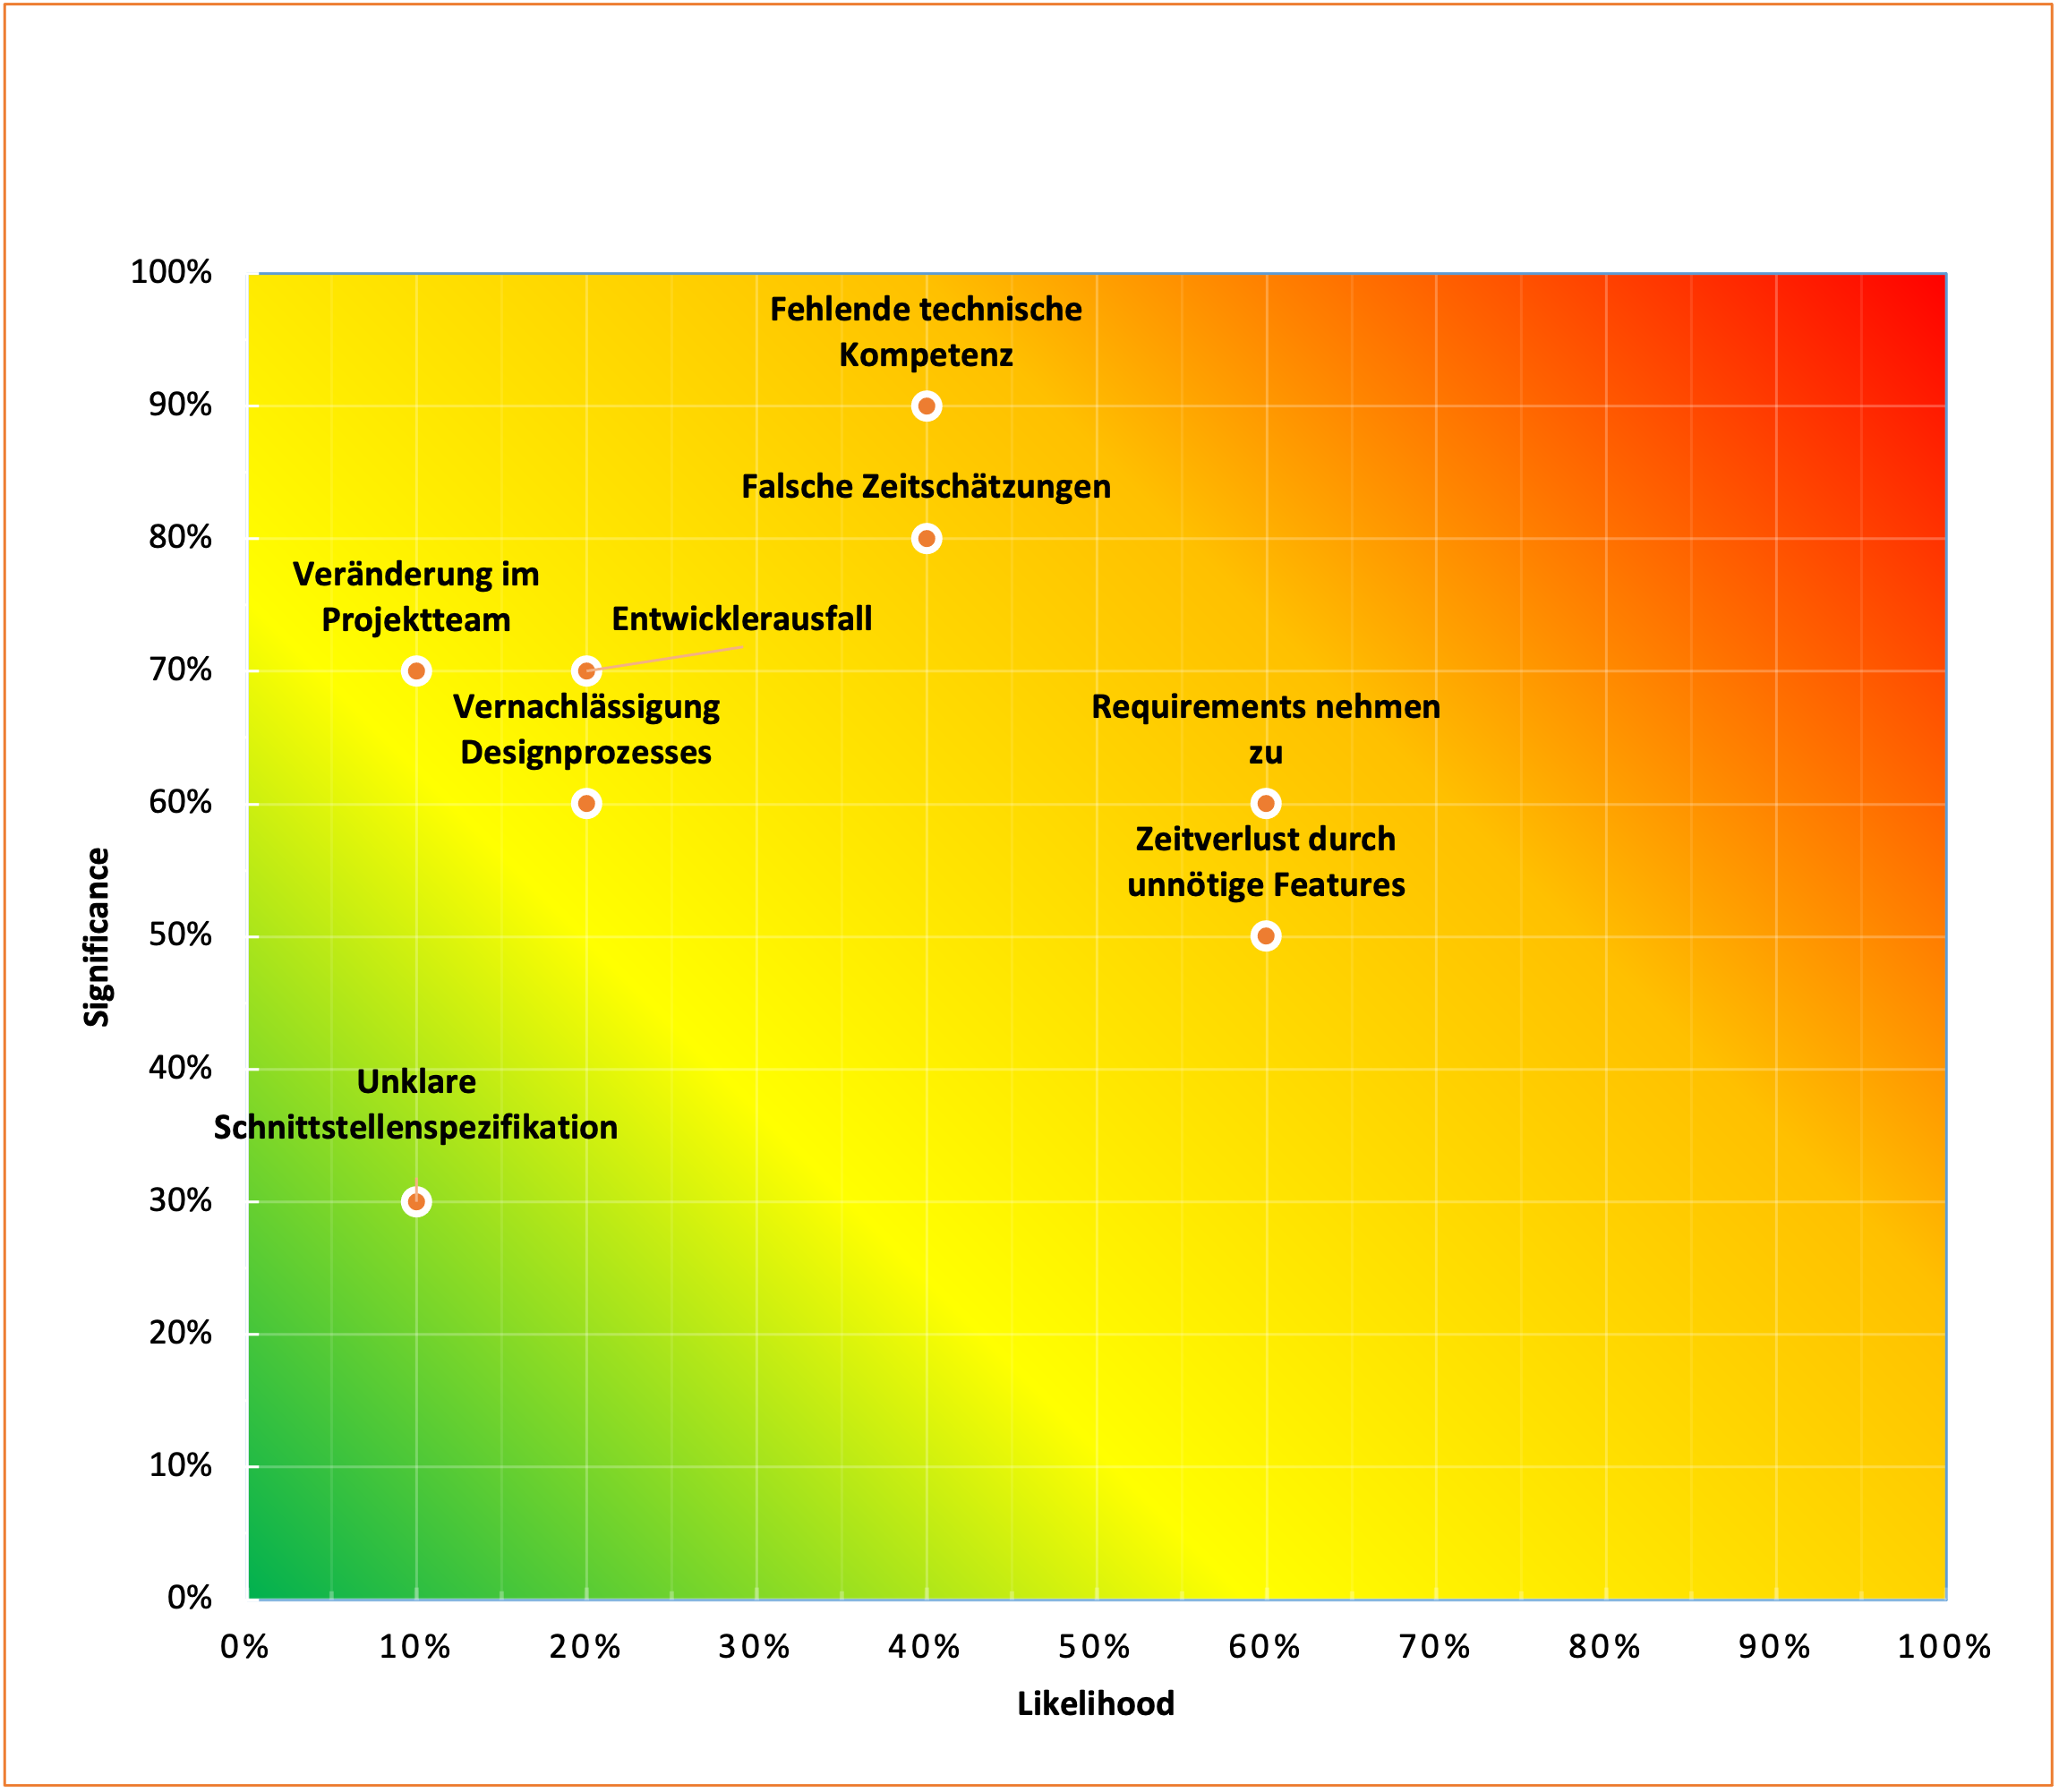
\includegraphics[width=1\textwidth]{bilder/RiskMap.png}
    \caption[Risikomatrix]{Risikomatrix,\\ Quelle: Autoren}
    \label{img: Risikomatrix}
\end{figure}

\paragraph{Beschreibung}
Basierend auf der Risikomatrix in Abbildung \ref{img: Risikomatrix} müssen für die Risiken im rechten oberen Viertel Gegenmassnahmen erarbeitet werden. Dabei handelt es sich um die folgenden Risiken:
\begin{itemize}
\item Falsche Zeiteinschätzung
\item Requirements nehmen zu/Veränderung der Requirements
\item Zeitverlust durch unnötige Features
\item Fehlende technische Kenntnisse
\end{itemize}

\paragraph{Gegenmassnahmen}
\subparagraph{Falsche Zeiteinschätzung}
Um das Risiko einer falschen Zeiteinschätzung zu minimieren wird bei der Planung auf bestehende, erfolgreich abgeschlossene Projekte zurückgegriffen. Basierend auf diesen wird die Zeitplanung durchgeführt.  
\subparagraph{Requirements nehmen zu/Veränderung der Requirements}
Die Requirements werden fortlaufend im Product Backlog überprüft. Die Aufgabenstellung dient dabei als Basis. Mittels vom Product Owner abgesegneten Akzeptanzkriterien ist der Umfang klar abgegrenzt. 
 \subparagraph{Zeitverlust durch unnötige Features}
Durch den Product Backlog sowie den Sprint Backlog mit klaren Beschreibungen sowie Akzeptanzkriterien der Issues sind dem Entwickler zu jedem Zeitpunkt die zu bearbeitenden Punkte klar.
 \subparagraph{Fehlende technische Kenntnisse}
Beim Projekt wird auf vielgenutzte Technologien mit grosser Community gesetzt. 

\begin{table}[H]
\begin{tabularx}{\textwidth}{|C|C|C|}
\hline
\textbf{Risiko} & \textbf{Eintrittswahrsch.} & \textbf{Schaden} \\
\hline
Falsche Zeiteinschätzung &  30 & 80\\
\hline
Requirements nehmen zu / Requirements ändern sich & 20 & 10\\
\hline
Zeitverlust unnötige Features & 30 & 50\\
\hline
Fehlende technische Kenntnisse & 40 & 40\\
\hline
\end{tabularx}
\caption{ \label{tbl: RisikoanalyseNachMassnahmen}Risikoanalyse nach Massnahmen, Quelle: Autoren}
\end{table}

\begin{figure}[H]
    \centering
    %\includegraphics[width=1\textwidth]{bilder/RiskMap_nachher.png}
    \caption[RisikomatrixNach]{Risikomatrix nach Massnahmen,\\ Quelle: Autoren}
    \label{img: RisikomatrixNachher}
\end{figure}

\subsubsection{Definition of done}
In jedem Sprint müssen die nachfolgenden Punkte zwingend erreicht werden, um ein potenziell auslieferbares Produkt zu erhalten:

\begin{itemize}
\item Review durchgeführt
\item Akzeptanzkriterien erfüllt
\item Unit Tests Grün
\item CI/CD ohne Fehler
\item keine kritischen Bugs
\item Clean Code Guidelines eingehalten
\item Dokumentation aktuell
\end{itemize}
\newpage
\subsection{Projektunterst\"utzung}
\subsubsection{Tools f\"ur Entwicklung, Test und Abnahme}
\paragraph{Entwicklungstools}
Bei der Entwicklung des Projekts kommen folgende Programme zum Einsatz: 

\begin{table}[H]
\setlength\extrarowheight{2pt} % for a bit of visual "breathing space"
\begin{tabularx}{\textwidth}{|C|C|C|}
\hline
\textbf{Typ} &\textbf{Tool} & \textbf{Version}  \\

\hline
IDE & Intelij Ultimate  & 2020.1\\
\hline
IDE & Webstorms & 2020.2\\ 
\hline
Versionsverwaltung & Git & 2.27.0\\
\hline
\end{tabularx}
\caption{ \label{tbl: Entwicklungstools}Entwicklungstools, Quelle: Autoren}
\end{table}
\paragraph{Testtools}
Beim Testing kommen folgende Tools zum Einsatz

\begin{table}[H]
\setlength\extrarowheight{2pt} % for a bit of visual "breathing space"
\begin{tabularx}{\textwidth}{|C|C|C|}
\hline
\textbf{Typ} &\textbf{Tool} & \textbf{Version}  \\
\hline
Unit Testing & JUnit  & 5.6.2\\
\hline 
API Testing & Postman & 7.36.0\\
\hline
\end{tabularx}
\caption{ \label{tbl: Testtools}Testtools, Quelle: Autoren}
\end{table}
\subsubsection{Konfigurationsmanagement}
\paragraph{Konfigurationseinheit}

Bei diesem Projekt besteht eine Konfigurationseinheit aus mehreren Teilen. Dabei werden diese bei jedem Release aufgeführt. Zusätzlich dazu kommen noch die Reports der Automatisierten Tests, falls vorhanden auch der Systemtests.
\begin{itemize}
\item API
\item Datenbank
\item Webapplikation
\item Dokument
\end{itemize}
\paragraph{Release 1}

\begin{table}[H]
\setlength\extrarowheight{2pt} % for a bit of visual "breathing space"
\begin{tabularx}{\textwidth}{|C|C|C|}
\hline
\textbf{Typ} &  \textbf{Version}  \\

\hline
API &  1.0.0\\
\hline
Datenbank &  1.0.0\\
\hline
Webapplikation  & 1.0.0\\
\hline
Dokumentation & 0.9\\
\hline
\end{tabularx}
\caption{ \label{tbl: Konfigurationseinheit Release 1}Konfigurationseinheit Release 1, Quelle: Autoren}
\end{table}

\paragraph{Testprotokolle}
Die gesamten Testprotokolle sind im Anhang \ref{Testprotokolle} zu finden. 
\newpage
\subsection{Teststrategie und Drehbuch}
\subsubsection{Teststrategie}
Es wird bei diesem Projekt hauptsächlich auf Automated Testing gesetzt.
Unit Tests werden dabei Integration Tests vorgezogen.
Hierzu wird auf das bewährte JUnit Framework gesetzt.
Es wird dabei das Test-First-Prinzip verwendet.

\paragraph{Automated Testing der REST-Schnittstelle}
Zum Testen der Rest-Schnittstelle wird Unirest sowie JUnit verwendet.  


\subsubsection{Testdrehbuch}\label{testsvonmeilensteine}
Wie oben genannt wird hautpsächlich auf Automated Testing gesetzt.
Daher werden nur sehr wenige manuelle Tests durchgeführt.
Die Tests gehen mit den gleichnamigen Meilensteinen einher.
Nachfolgend werden diese inklusive den erhaltenen Resultate beschrieben.

\begin{table}[H]
\begin{tabularx}{\textwidth}{lX}
  \hline
  \multicolumn{2}{|c|}{Test Lernmodus Frage anzeigen} \\
  \hline
  Test Nr. & 1\\
  Beschreibung & Durch diesen Test wird die Lernfunktion sowie die Lernstatistik für Lernende manuell getestet.\\
  Randbedingungen & Die Testperson hat einen bereits eingerichteten Account mit den für sie relevanten Fragen.\\
  erwartete Resultate & Der Nutzer bekommt eine Frage inklusive den möglichen Antworten angezeigt.  \\
  Testperson & Frederico Fischer \\
  Datum & 01.10.2020 \\
  Testprotokoll & \ref{tbl: testprotokoll1}\\
   \hline
\end{tabularx}
\caption{ \label{tbl: Test Lernmodus Frage anzeigen}Test Lernmodus Frage anzeigen, Quelle: Autoren}
\end{table}


\begin{table}[H]
\begin{tabularx}{\textwidth}{lX}
  \hline
  \multicolumn{2}{|c|}{Test Lernmodus Frage beantworten} \\
  \hline
  Test Nr. & 2\\
  Beschreibung & Durch diesen Test wird die Beantwortung von Fragen getestet.\\
  Randbedingungen & Die Testperson hat einen bereits eingerichteten Account mit für sie relevanten Fragen. Der Test Nr. 1 ist erfolgreich verlaufen\\
  erwartete Resultate & Der Nutzer kann eine Fragen beantworten und gelangt direkt zur nächsten.  \\
  Testperson & Frederico Fischer \\
  Datum & 01.10.2020 \\
  Testprotokoll & \ref{tbl: testprotokoll2}\\
   \hline
\end{tabularx}
\caption{ \label{tbl: Test Lernmodus Frage beantworten}Test Lernmodus Frage anzeigen, Quelle: Autoren}
\end{table}

\begin{table}[H]
\begin{tabularx}{\textwidth}{lX}
  \hline
  \multicolumn{2}{|c|}{Test Lernmodus Frage korrigieren} \\
  \hline
  Test Nr. & 3\\
  Beschreibung & Durch diesen Test wird die Korrektur von Fragen getestet.\\
  Randbedingungen & Die Testperson hat einen bereits eingerichteten Account mit für sie relevanten Fragen. Die Tests Nr. 1 und 2 sind erfolgreich verlaufen\\
  erwartete Resultate & Bei der Beantwortung der Frage wird dem Nutzer angezeigt, ob die angewählte Lösung korrekt war. Falls nicht, wird die richtige Lösung angezeigt.  \\
  Testperson & Frederico Fischer \\
  Datum & 01.10.2020 \\
  Testprotokoll & \ref{tbl: testprotokoll3}\\
   \hline
\end{tabularx}
\caption{ \label{tbl: Test Lernmodus Frage korrigieren}Test Lernmodus Frage korrigieren, Quelle: Autoren}
\end{table}

\begin{table}[H]
\begin{tabularx}{\textwidth}{lX}
  \hline
  \multicolumn{2}{|c|}{Test Lernmodus Statistik zu User anzeigen} \\
  \hline
  Test Nr. & 4\\
  Beschreibung & Durch diesen Test wird die Anzeige einer Userstatistik gestestet.\\
  Randbedingungen & Es sind bereits 3 Statistiken zu unterschiedlichen Fragen in der Datenbank vorhanden. \\
  erwartete Resultate & Dem Nutzer wird seine Nutzerstatistik bezogen auf die beantworteten Fragen angezeigt.  \\
  Testperson & Frederico Fischer \\
  Datum & 01.12.2020 \\
  Testprotokoll & \ref{tbl: testprotokoll4}\\
   \hline
\end{tabularx}
\caption{ \label{tbl: Test Lernmodus Statistik anzeigen}Test Lernmodus Statistik anzeigen, Quelle: Autoren}
\end{table}

\begin{table}[H]
\begin{tabularx}{\textwidth}{lX}
  \hline
  \multicolumn{2}{|c|}{Test Registrierung} \\
  \hline
  Test Nr. & 5\\
  Beschreibung & Durch diesen Test wird die Registrierung eines neuen Nutzers getestet \\
  Randbedingungen & Ein Nutzer mit diesem Benutzernamen ist noch nicht erstellt worden. \\
  erwartete Resultate & Auf dem Bildschirm wird die Meldung "User created successfully" angezeigt.  \\
  Testperson & Frederico Fischer \\
  Datum & 01.10.2020 \\
  Testprotokoll & \ref{tbl: testprotokoll5}\\
   \hline
\end{tabularx}
\caption{ \label{tbl: Test Registrierung}Test Registrierung, Quelle: Autoren}
\end{table}

\begin{table}[H]
\begin{tabularx}{\textwidth}{lX}
  \hline
  \multicolumn{2}{|c|}{Test Login} \\
  \hline
  Test Nr. & 6\\
  Beschreibung & Durch diesen Test wird das Login eines Nutzers getestet \\
  Randbedingungen & Ein Nutzer mit dem Benutzernamen \flqq peterpan\frqq und dem Passwort \flqq peterpan\frqq ist erfolgreich erstellt worden. \\
  erwartete Resultate & Der Nutzer wird erfolgreich angemeldet. Im Userprofil wird der korrekte Nutzer angezeigt.   \\
  Testperson & Frederico Fischer \\
  Datum & 01.10.2020 \\
  Testprotokoll & \ref{tbl: testprotokoll6}\\
   \hline
\end{tabularx}
\caption{ \label{tbl: Test Einloggen}Test Einloggen, Quelle: Autoren}
\end{table}

\begin{table}[H]
\begin{tabularx}{\textwidth}{lX}
  \hline
  \multicolumn{2}{|c|}{Test Zugriff geschütze Ressource} \\
  \hline
  Test Nr. & 7\\
  Beschreibung & Durch diesen Test wird der  Zugriff auf eine geschützte Ressource getestet.  \\
  Randbedingungen & Ein Nutzer mit dem Benutzernamen "peterpan" und dem Passwort "peterpan" ist erfolgreich angemeldet worden. \\
  erwartete Resultate & Der Nutzer greift auf die Lernfunktion zu. Er kann mit einer Lernsession beginnen.   \\
  Testperson & Frederico Fischer \\
  Datum & 01.12.2020 \\
  Testprotokoll & \ref{tbl: testprotokoll7}\\
   \hline
\end{tabularx}
\caption{ \label{tbl: Test Login}Test Zugriff geschütze Ressource, Quelle: Autoren}
\end{table}

\begin{table}[H]
\begin{tabularx}{\textwidth}{lX}
  \hline
  \multicolumn{2}{|c|}{Test Aufgabenstellung hinzufügen} \\
  \hline
  Test Nr. & 8\\
  Beschreibung & Durch diesen Test wird das Hinzufügen einer neuen Aufgabenstellung im Multiple Choice Format getestet. \\
  Randbedingungen & Es wird ein bereits eingerichteter Lehreraccount,  bestehende CategorySets und Categories, sowie die vorhandenen Bilder zur Verfügung gestellt. \\
  erwartete Resultate &  Die Frage wird erstellt und dem gewünschten CategorySet hinzugefügt. \\
  Testperson & Frederico Fischer \\
  Datum & 01.12.2020 \\
  Testprotokoll & \ref{tbl: testprotokoll8}\\
   \hline
\end{tabularx}
\caption{ \label{tbl: Test Aufgabenstellung hinzufuegen}Test Aufgabenstellung hinzufügen,  Quelle: Autoren}
\end{table}

\begin{table}[H]
\begin{tabularx}{\textwidth}{lX}
  \hline
  \multicolumn{2}{|c|}{Test Prüfung aus bestehenden Fragen erstellen} \\
  \hline
  Test Nr. & 9\\
  Beschreibung & Durch diesen Test wird das Erstellen und direkte Freigeben einer Prüfung getestet. \\
  Randbedingungen & Es wird ein bereits eingerichteter Lehreraccount,  bestehende CategorySets und Categories,  Schulklassen mit Schülern,  sowie die vorhandenen Bilder zur Verfügung gestellt. \\
  erwartete Resultate &  Die Prüfung kann mit den gewünschten Fragen und den gewählten Klassen erstellt werden.  \\
  Testperson & Frederico Fischer \\
  Datum & 01.12.2020 \\
  Testprotokoll & \ref{tbl: testprotokoll9}\\
   \hline
\end{tabularx}
\caption{ \label{tbl: Test Pruefung erstellen}Test Prüfung erstellen,  Quelle: Autoren}
\end{table}

\begin{table}[H]
\begin{tabularx}{\textwidth}{lX}
  \hline
  \multicolumn{2}{|c|}{Test Analysieren und bearbeiten einer abgeschlossenen Prüfung} \\
  \hline
  Test Nr. & 10\\
  Beschreibung & Durch diesen Test wird das nachträgliche Bearbeiten von Prüfungsresultaten durch einen Lehrer getestet. \\
  Randbedingungen & Es wird ein bereits eingerichteter Lehreraccount mit einer von Schülern absolvieren Prüfung zur Verfügung gestellt.  \\
  erwartete Resultate & Der Lehrer kann die Antworten von einzelnen Usern dessen Fragen bearbeiten und so die erreichte Punktezahl korrigieren.   \\
  Testperson & Frederico Fischer \\
  Datum & 01.12.2020 \\
  Testprotokoll & \ref{tbl: testprotokoll10}\\
   \hline
\end{tabularx}
\caption{ \label{tbl: Test Analysieren und bearbeiten einer abgeschlossenen Pruefung}Test Analysieren und bearbeiten einer abgeschlossenen Prüfung, Quelle: Autoren}
\end{table}

\begin{table}[H]
\begin{tabularx}{\textwidth}{lX}
  \hline
  \multicolumn{2}{|c|}{Test Absolvieren einer Prüfung nur während bestimmtem Zeitraum} \\
  \hline
  Test Nr. & 11\\
  Beschreibung & Durch diesen Test wird das Absolvieren einer Prüfung ausserhalb eines gültigen Zeitraums getestet. \\
  Randbedingungen & Es ist eine Prüfung mit einem Bearbeitungszeitraum vom 1.1.2020 - 2.1.2020 erstellt worden. Die Prüfung wurde der Klasse des Users freigegeben.  \\
  erwartete Resultate & Der Schüler kann die Prüfung nicht starten.  \\
  Testperson & Frederico Fischer \\
  Datum & 01.12.2020 \\
  Testprotokoll & \ref{tbl: testprotokoll11}\\
   \hline
\end{tabularx}
\caption{ \label{tbl: Test Absolvieren einer Pruefung nur waehrend bestimmtem Zeitpunkt}Test Absolvieren einer Prüfung nur während bestimmtem Zeitpunkt, Quelle: Autoren}
\end{table}

\begin{table}[H]
\begin{tabularx}{\textwidth}{lX}
  \hline
  \multicolumn{2}{|c|}{Test Absolvieren einer Prüfung ohne Berechtigung} \\
  \hline
  Test Nr. & 12\\
  Beschreibung & Durch diesen Test wird das Absolvieren einer Prüfung für einen nicht authorisierten Nutzer getestet.  \\
  Randbedingungen & Es ist eine Prüfung mit einem gütigen Bearbeitungszeitraum erstellt worden. Die Testperson besitzt einen Schüleraccount, für den die entsprechende Prüfung nicht zugewiesen wurde.  \\
  erwartete Resultate & Die Testperson kann die Prüfung nicht starten.  \\
  Testperson & Frederico Fischer \\
  Datum & 01.12.2020 \\
  Testprotokoll & \ref{tbl: testprotokoll12}\\
   \hline
\end{tabularx}
\caption{ \label{tbl: Test Absolvieren einer Pruefung ohne Berechtigungen}Test Absolvieren einer Prüfung ohne Berechtigungen, Quelle: Autoren}
\end{table}

\begin{table}[H]
\begin{tabularx}{\textwidth}{lX}
  \hline
  \multicolumn{2}{|c|}{Test Migration von Daten} \\
  \hline
  Test Nr. & 13\\
  Beschreibung & Durch diesen Test wird die Migration der Daten in die neue Applikation getestet.  \\
  Randbedingungen & Die bestehende Datenbank wurde gelöscht und die Applikation neu gestartet.  Die csv-Dateien werden mit den zur Verfügung gestellten Postman Kommandos an die API gesendet.  \\
  erwartete Resultate & Die Daten werden erfolgreich in die Applikation migriert.  Bei der Migration der Fragen ist nach Auftreten einer Fehlermeldung ein erneutes Senden nötig. In der Datenbank befinden sich rund 3000 Fragen. \\
  Testperson & Frederico Fischer \\
  Datum & 01.12.2020 \\
  Testprotokoll & \ref{tbl: testprotokoll13}\\
   \hline
\end{tabularx}
\caption{ \label{tbl: Test Migration von Daten}Test Migration von Daten, Quelle: Autoren}
\end{table}
\newpage
